\chapter{Configuring Apache Virtual Hosts}

	\section{Understanding Apache Configuration Files}
The main configuration file for the apache web server is \verb|/etc/httpd/conf/httpd.conf|. Within this file, is a config called the \verb|ServerRoot|. All the file names defined within this file are relative to the \textit{ServerRoot}. 

\vspace{-15pt}
\begin{minted}{lighttpd}
ServerRoot "/etc/httpd"
\end{minted}
\vspace{-10pt}	

\noindent
Apache is modular in nature, which means different functionalities can be added as modules, instead of just one monolithic program. This means that each of these modules may need their own configuration specific to their functionality. The configuration files for the different modules are stored in \verb|/etc/httpd/conf.modules.d|. Further, with every new module that's included in the apache server running on a host, the folder might get a new config file for that module. 

The contents of the module config directory (\verb|/etc/httpd/conf.modules.d|) are added to the configuration of the web server by the include instruction in \verb|httpd.conf|:

\vspace{-15pt}
\begin{minted}{lighttpd}
Include conf.modules.d/*.conf
\end{minted}
\vspace{-10pt}	

\noindent
This folder contains files that aid primarily in the loading of appropriate modules from the \verb|/usr/lib/httpd/modules| directory, which has a softlink in \verb|/etc/httpd/modules|. The directory structure of the httpd directory is:

\vspace{-15pt}
\begin{minted}{console}
# ls -l /etc/httpd
total 0
drwxr-xr-x. 2 root root  37 Mar  7 22:48 conf
drwxr-xr-x. 2 root root  82 Mar  7 22:37 conf.d
drwxr-xr-x. 2 root root 146 Mar  7 22:37 conf.modules.d
lrwxrwxrwx. 1 root root  19 Mar  7 22:37 logs -> ../../var/log/httpd
lrwxrwxrwx. 1 root root  29 Mar  7 22:37 modules -> ../../usr/lib64/httpd/modules
lrwxrwxrwx. 1 root root  10 Mar  7 22:37 run -> /run/httpd
\end{minted}
\vspace{-10pt}	

\noindent
In addition to all the above, files in the \verb|/etc/httpd/conf.d| directory that end with a \verb|.conf| extension will also automatically be included in the apache configuration. The files in this directory are included optionally in \verb|httpd.conf| using:

\vspace{-15pt}
\begin{minted}{lighttpd}
IncludeOptional conf.d/*.conf
\end{minted}
\vspace{-10pt}	

\noindent
This directory is primarily used by the plugin files from RPMs. (eg. httpd-manual). Apache is also configured to use a default document root at \verb|/var/www/html|. This is the directory that serves as the base directory of the website being hosted on the web server. The default \textit{DocumentRoot} is configured in \verb|httpd.conf| using:

\vspace{-15pt}
\begin{minted}{lighttpd}
DocumentRoot "/var/www/html"
\end{minted}
\vspace{-10pt}	

\section{Exploring the httpd.conf file}
The \verb|listen| directive tells the Apache web server which IP address and port to listen on for incoming connections. This can take two forms:

\vspace{-15pt}
\begin{minted}{lighttpd}
# Listen 12.34.56.78:80
Listen 80
\end{minted}
\vspace{-10pt}	

\noindent
In the first example we are instructing the Apache web server's http daemon to listen for incoming connections only on port \verb|80| of the IP address \verb|12.34.56.78|. In case of multiple network interfaces connected to the host running the web server, only the host with the IP address \verb|12.34.56.78| will be able to provide incoming connections. However, if we were to omit the IP address, then the httpd process will listen on port 80 for every IP address associated with the network interfaces on the server. For obvious reasons, one of these directives need to stay commented out while the other is active. 

Further down, there's the \textit{user} and \textit{group} parameter, which determines the user and group as which the Apache web server is run with. 

\vspace{-15pt}
\begin{minted}{lighttpd}
User apache
Group apache
\end{minted}
\vspace{-10pt}	

\noindent
The apache process runs under the apache user and apache group, and thus if any security in the website is exploited and someone gains unauthorized access, they can gain a minimal amount of power since the apache user is given minimal privileges. Next, the location of the error logs is set in the parameter:

\vspace{-15pt}
\begin{minted}{lighttpd}
ErrorLog "logs/error_log"
...
LogLevel warn
\end{minted}
\vspace{-10pt}	

\noindent
Since the location is relative, the absolute location for a \textit{ServerRoot} of \verb|/etc/httpd| is: \verb|/etc/httpd/logs/error_log|. 

\subsection{Directory access rules}
The \verb|httpd.conf| file contains several \verb|<Directory>| tags that determine the kind of access the web server has over certain directories. For example, the \verb|/var/www| directory, i.e., the parent directory of the \textbf{DocumentRoot} has the following rules associated to it:

\vspace{-15pt}
\begin{minted}{lighttpd}
<Directory "/var/www">
	AllowOverride None
	# Allow open access:
	Require all granted
</Directory>
\end{minted}
\vspace{-10pt}	

\noindent
The \verb|AllowOverride| directive decides what kind of information may be contained within \verb|.htaccess| files which are used to customize the kind of permission each directory has on a granular level. When a \verb|.htaccess| file is encountered, based on the values in the \verb|<Directory>| tags for that folder, certains settings from the \verb|.htaccess| files will override the original settings in the config files. 

The \verb|Require| directive is used to determine who has access to visit the directory using HTTP/HTTPS through the website. For example, the \verb|Require all granted| statement means that anyone from any IP can visit the contents of this directory. \verb|Require all denied| mean the directory is inaccessible via the web server. Additionally, the \verb|Require ip 10.0.50.99| would only allow the mentioned IP to access the contents of that directory. Similarly, the \verb|Require host example.org| statement would allow hosts on the \textit{example.org} domain to access the directory contents, while denying all other hosts, and so on.

\vspace{-15pt}
\begin{minted}{lighttpd}
Options Indexes FollowSymLinks
\end{minted}
\vspace{-10pt}	

The \verb|Options| directive controls which features of the Apache server are available in a particular directory. For example, \verb|Options FollowSymLinks| would let the httpd process follow symlinks in the concerned directory. Similarly, the \verb|Options Indexes| makes the server present a formatted list of directory content when an index.html page is not found in the folder corresponding to the URL. 

\section{Configuring a simple Web Server}
Configuring a basic web server is simple, but it does take a bit of prep work. First, we must install the Apache web server which provides the http daemon, and comes in the package \verb|httpd|. Now, by default the service \verb|httpd| isn't started. So, we need to enable and start it. Then, we need to open the appropriate firewall ports (\verb|80| for HTTP, \verb|443| for HTTPS). Then, we can ensure that the web server is operational by visiting the \verb|http://localhost| site, where we should see a distro specific welcome page for the web server.

\vspace{-15pt}
\begin{minted}{console}
# yum -y install httpd
# systemctl enable httpd; systemctl start httpd
# firewall-cmd --add-service=http --add-service=https --permanent
# firewall-cmd --reload
# yum -y install elinks
# elinks http://localhost
\end{minted}
\vspace{-10pt}	

\noindent
Now, we can go to the \textit{DocumentRoot} (\verb|/var/www/html| by default) and create a file called \verb|index.html| and see if we can access it from our browser by going to the localhost site (\verb|http://localhost|). The contents of the index.html file should contain valid html like:

\vspace{-15pt}
\begin{minted}{html}
<html>
	<head>
		<title>Test Page!</title>
	</head>
	<body>
		<h1>Success!</h1>
		<p>The Web Server at vmPrime is now operational!</p>
	</body>
</html>
\end{minted}
\vspace{-10pt}	

\subsection{Changing DocumentRoot}
Let's now create an index.html file within a \verb|/var/www/html/web| directory:

\vspace{-15pt}
\begin{minted}{console}
# mkdir /web
# cd /web
# vim index.html
\end{minted}
\vspace{-10pt}	

\noindent
Inside the index.html, we put the contents:

\vspace{-15pt}
\begin{minted}{html}
<html>
	<head>
		<title>Subdirectory Test Page!</title>
	</head>
	<body>
		<h1>Success!</h1>
		<p>You're now visiting a subdirectory in the DocumentRoot</p>
	</body>
</html>
\end{minted}
\vspace{-10pt}	

\noindent
To make this the new homepage within our site, we need to change the \textit{DocumentRoot} in httpd.conf and then adjust the SELinux contexts. The \verb|/etc/httpd/conf/httpd.conf| file will need to have the original DocumentRoot specification deleted/commented out, and have the new lines added:

\vspace{-15pt}
\begin{minted}{lighttpd}
# DocumentRoot "/var/www/html"
DocumentRoot "/web"
<Directory "/web">
	Options Indexes FollowSymLinks
	AllowOverride None
	Require all granted
</Directory>
\end{minted}
\vspace{-10pt}	

\subsection{Dealing with SELinux Security Context}
Now, we need to deal with the SELinux contexts. Since the new DocumentRoot is in \verb|/web| and not a child of \verb|/var/www/hmtl|, it'll have a different SELinux security context. This needs to be fixed for the httpd process to be able to access it. The default security context can be seen with:

\vspace{-15pt}
\begin{minted}{console}
# ls -ldZ /web
drwxr-xr-x. root root unconfined_u:object_r:default_t:s0 /web
# ls -ldZ /var/www/html
drwxr-xr-x. root root system_u:object_r:httpd_sys_content_t:s0 /var/www/html
\end{minted}
\vspace{-10pt}	

\noindent
We can see that the security context for the folders are different, which will trigger SELinux to block the httpd process. In case the correct context is not know, we use the command \verb|semanage fcontext -l | grep <processName|originalPath>| to determine the right context:
AllowOverride None
Require all granted	
\vspace{-15pt}AllowOverride None
Require all granted	
\begin{minted}{console}
# semanage fcontext -l | grep /var/www
/var/www(/.*)?        all files        system_u:object_r:httpd_sys_content_t:s0 
\end{minted}
\vspace{-10pt}	

\noindent
We have now confirmed the security context should be \verb|httpd_sys_content_t|. Now, to apply it to the \verb|/web| directory, we again use \verb|semanage fcontext|: 

\vspace{-15pt}
\begin{minted}{console}
# semanage fcontext -a -t httpd_sys_content_t "/web(/.*)?"
# restorecon -Rv /web
restorecon reset /web context unconfined_u:object_r:default_t:s0->unconfined_u:object_r:httpd_sys_content_t:s0
\end{minted}
\vspace{-10pt}	

\noindent
The \verb|restorecon| command recursively rectifies the contexts according to the security context of the \verb|/web| directory. Since our original RegEx for the file selection in the \verb|semanage| command was \verb|/web(/.*?)|, i.e., \verb|/web| and all it's children, the \verb|restorecon| commands applies the \verb|httpd_sys_content_t| context to everything under the \verb|/web| directory. Now we just restart the \verb|httpd| service for the changes in \verb|/etc/httpd/conf/httpd.conf| to take effect:

\vspace{-15pt}
\begin{minted}{console}
# sysmtectl restart httpd
# elinks http://localhost
\end{minted}
\vspace{-10pt}	

\subsection{Giving Web Developers access to the new DocumentRoot}
The developers need read-write access on the \verb|/web| directory for it to be of any use. However, since it's a directory directly inside the \verb|/| directory, and due to a host of other security reasons, it's a bad idea to make them owners of the directory. We could create a \textit{webdev} group and make them the group owner, but this approach is limited since only one group can be the group owner of a directory. If some other group also needs access, then this method fails. So, the best way to deal with this is to use Access Control Lists (ACLs). We can get the default ACL by:

\vspace{-15pt}
\begin{minted}{console}
# getfacl /web
getfacl: Removing leading '/' from absolute path names
# file: web
# owner: root
# group: root
user::rwx
group::r-x
other::r-x
\end{minted}
\vspace{-10pt}	

\noindent
First of all, we need to create a group for the web developers. Then, since we have to create an ACL for a directory, we need two sets: one for the existing files in the directory (and the directory itself) as well as a default ACL for any files that are created in the future. So, we use:

\vspace{-15pt}
\begin{minted}{console}
# groupadd webdev
# chmod -R u=rwX,go=rX /web
[root@vmPrime web]# ls -l /web; ls -ld /web
total 4
-rw-r--r--. 1 root root 165 Mar  8 12:29 index.html
drwxr-xr-x. 2 root root 24 Mar  8 12:34 /web
[root@vmPrime web]# setfacl -R -m g:webdev:rwX /web
[root@vmPrime web]# setfacl -R -m d:g:webdev:rwX /web
[root@vmPrime web]# getfacl /web
getfacl: Removing leading '/' from absolute path names
# file: web
# owner: root
# group: root
user::rwx
group::r-x
group:webdev:rwx
mask::rwx
other::r-x
default:user::rwx
default:group::r-x
default:group:webdev:rwx
default:mask::rwx
default:other::r-x
\end{minted}
\vspace{-10pt}	

\noindent
Note the use of capital \textbf{X} in the permissions (\textbf{rwX})- which means only the directories should be given execute permissions, (i.e., the user/group/others) can visit it. The execution permissions of the files are not touched, thus they remain executable if they already were, but if they weren't, they still aren't made executable. 

Now, each new file and directory within \verb|/web| as well as the existing ones are accessible with read-write permissions to the members of the group \textit{webdev}. In case any errors were made while setting the ACLs, the command \verb|setfacl -Rb /web| would remove any extended ACL so that we can try again!

\section{Introducing Virtual Hosts}
When looking for a particular website, a client requires name resolution either through a DNS query or domain name to IP mapping in \verb|/etc/hosts|. In either case, when a web server hosts multiple websites, they each are configured with a virtual host. Thus, a single httpd process may be managing many virtual hosts, each representing a website. 

\begin{figure}[H]
	\centering
	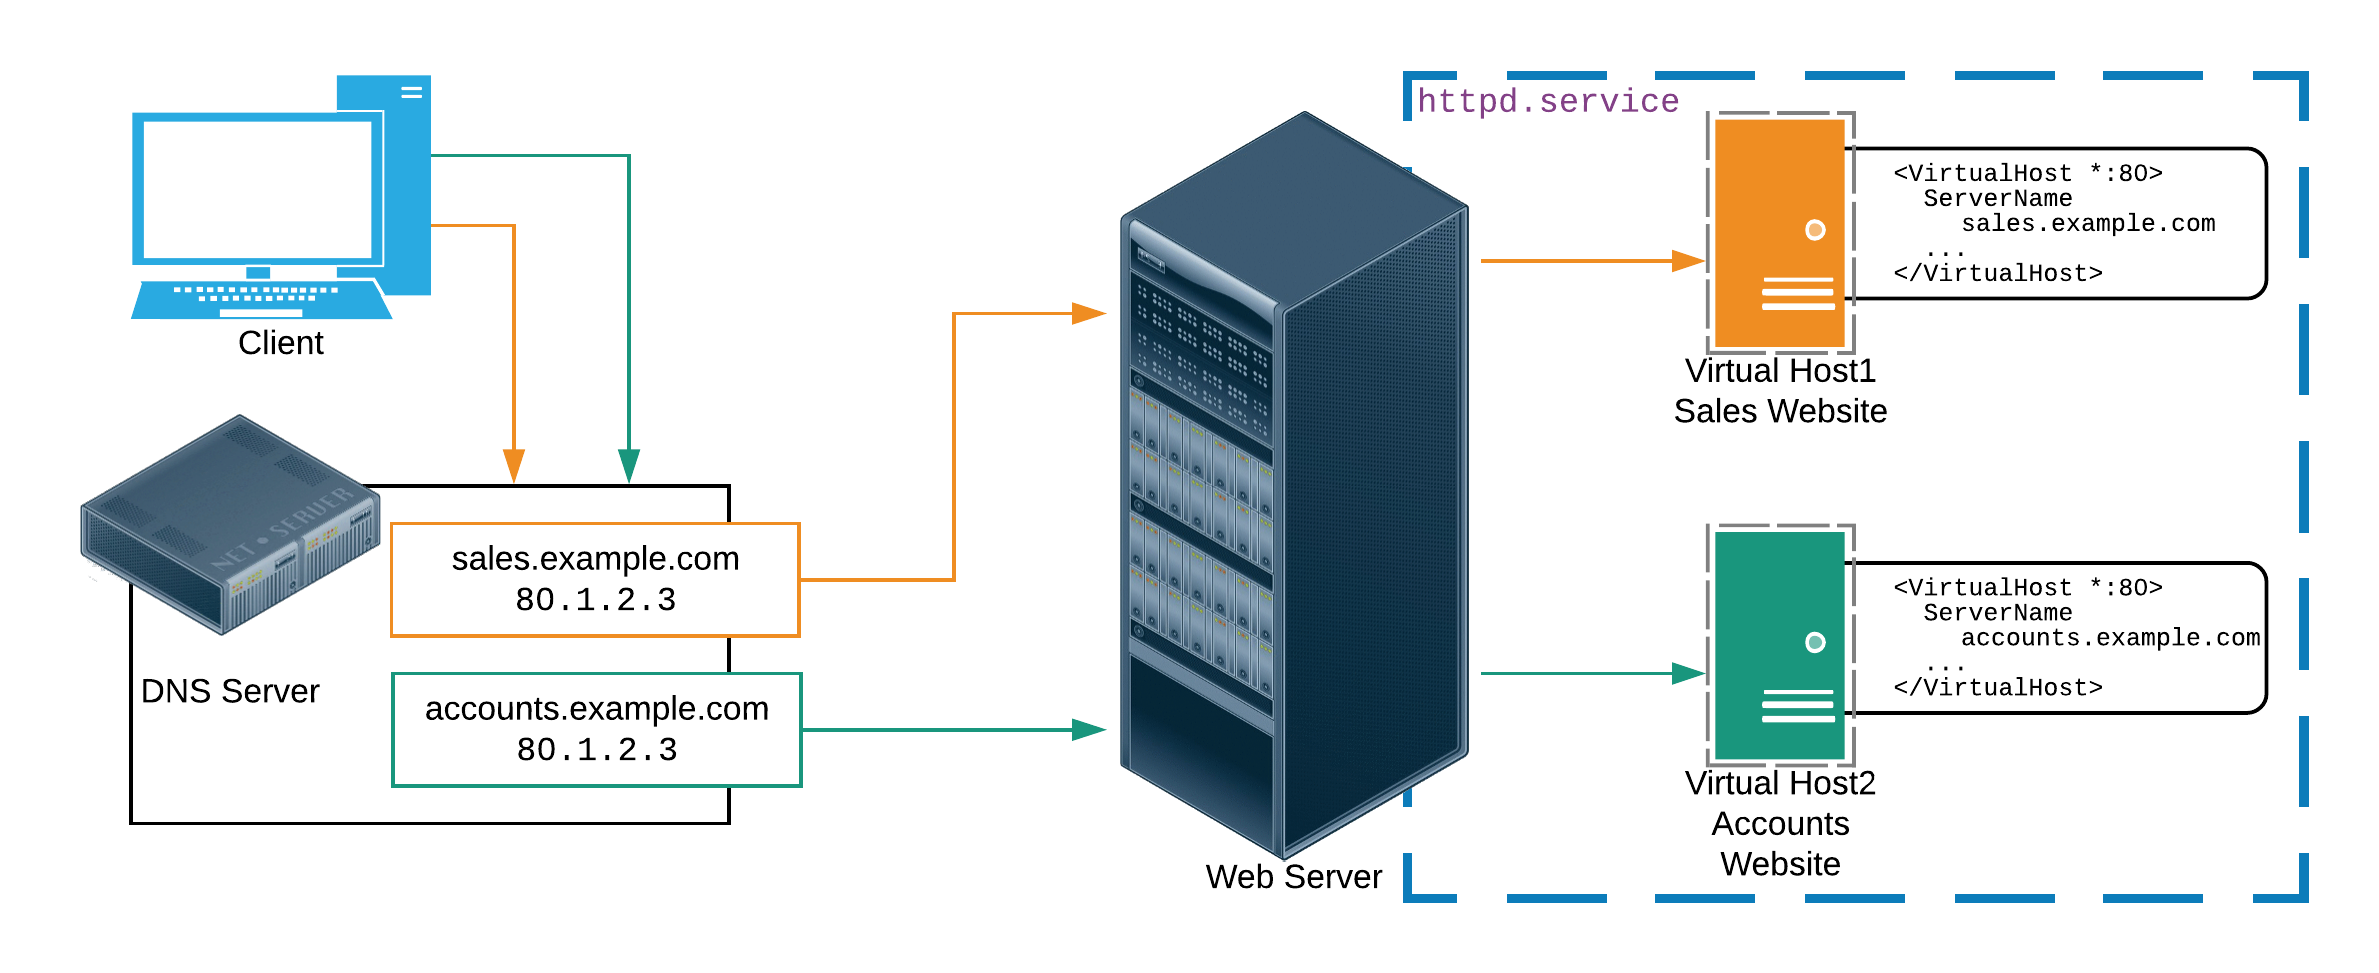
\includegraphics[width=\linewidth]{Mod2/chapters/2.8.a}
	\caption{Virtual Hosts}
	\label{fig:2}
\end{figure}

\noindent
Each of the virtual hosts are configured to run on the same IP address - in this particular process of virtual hosting, called \textbf{Name Based Virtual Hosting}. An alternative approach is called \textit{IP based Virtual Hosting}, where each virtual host is configured to use a different IP. However, in our case, all the virtual hosts use the same IP as assigned to the web server. The httpd process on the web server keeps listening on port 80 and the incoming packets are evaluated to determine which host the packet is addressed to, and then forwards it to that host. 

\section{Configuring Virtual Hosts}
To add a virtual host, we only need to add a couple of lines to the Apache configuration, and we can do that directly in the main config file \verb|httpd.conf|. While this approach works for a smaller number of virtual hosts, a better option is to create a \verb|.conf| file within the \verb|/etc/httpd/conf.d| directory and add our specifications for the virtual hosts in that file. Let us create two virtual hosts: \textit{sales} and \textit{accounts}, by creating \verb|sales.conf| and \verb|accounts.conf| in the aforementioned directory. The contents of \verb|sales.conf| will be:

\vspace{-15pt}
\begin{minted}{lighttpd}
<Directory /srv/web/sales>
	AllowOverride None
	Require all granted	
</Directory>

# Virtual Host settings:
<VirtualHost *:80>
	DocumentRoot /srv/web/sales						
	ServerName sales.somuVMnet.local
	ServerAlias salesSite.somuvmnet.local
	ServerAdmin root@sales.somuvmnet.local			
	ErrorLog "logs/sales_error_log"
	CustomLog "logs/sales_access_log" combined
</VirtualHost>
\end{minted}
\vspace{-10pt}	

\noindent
The first line of the virtual host configuration, \verb|<VirtualHost *:80>| asks the httpd process to listen for incoming connections for this virtual host on \textbf{all IPs(*)} instead of any specific IP on the port 80. The ServerAlias provides an alternate name for the server. The ServerAdmin is an email id that the webserver can send automated mail to. The ErrorLog is the location of the error log for this particular virtual host, since we wouldn't want to combine the error logs of several servers! Now, we set up name resolution by either a DNS server or by adding the line \verb|127.0.0.1  sales.somuVMnet.local| to the \verb|/etc/hosts| file. We also add a test web page in the \verb|/srv/web/sales| directory:

\vspace{-15pt}
\begin{minted}{html}
<html>
	<head>
		<title>Virtual Host Test Page!</title>
	</head>
	<body>
		<h1>Success!</h1>
		<p>Welcome to the sales dept homepage!!</p>
	</body>
</html>
\end{minted}
\vspace{-10pt}	

\noindent
Now, finally, we check the syntax of the config files using \verb|httpd -t|. This command is extremely useful because in a live production environment a bad config can bring down the web server as long as httpd refuses to restart. If the syntax is OK, we restart the webserver:

\vspace{-15pt}
\begin{minted}{console}
# httpd -t
Syntax OK
# systemctl restart httpd
\end{minted}
\vspace{-10pt}	

\noindent	
Once the above is done (assuming the SELinux context for \verb|/srv/web/sales| has been sorted out), the server should be reachable at \textit{sales.somuVMnet.local}. We confirm using \verb|elinks http://sales.somuVMnet.local|. If anything were to go wrong with the httpd, we could find the error logs for the server at \verb|/var/log/httpd/sales_error_log|. 

\subsection{Warnings}
Note that due to the use of the virtual host, the default HTTP configuration that we created for localhost is now non-operational, since the httpd process assumes any and all servers will now be presented as a virtual host.

Another side effect is that if a host can't be found, the httpd process presents the first virtual host that was configured irrespective of what the original query was. This can lead to massive confusion since one bad config can present enormous problems here! Now, httpd loads virtual hosts in an alphabetical order, and thus we can name a file \verb|00-errorHost.conf| and configure it to be a virtual host that shows an error message in perpetuity. 

\subsection{Creating a second virtual host on the same server}
Now, for the accounts department virtual host, we may choose to put it in the original DocumentRoot of our server at \verb|/web|. This means the config file for this virtual host won't need a \verb|<Directory>| tag. Thus, the config file for \verb|/etc/httpd/conf.d/accounts.conf| becomes:

\vspace{-15pt}
\begin{minted}{lighttpd}
# Virtual Host settings:
<VirtualHost *:80>
	ServerName accounts.somuVMnet.local
	ServerAlias acc.somuvmnet.local
	ServerAdmin root@accounts.somuvmnet.local			
	ErrorLog "logs/acc_error_log"
	CustomLog "logs/acc_access_log" combined
</VirtualHost>
\end{minted}
\vspace{-10pt}	

\noindent
We now need to create a web page in \verb|/web/index.html| that contains:

\vspace{-15pt}
\begin{minted}{html}
<html>
	<head>
		<title>Subdirectory Test Page!</title>
	</head>
	<body>
		<h1>Account Dept</h1>
		<p>You're now visiting accounts dept homepage!</p>
	</body>
</html>
\end{minted}
\vspace{-10pt}	

\noindent
We need to configure hostname resolution for the accounts website. So, we add to the \verb|/etc/hosts| files the line: \verb|127.0.0.1  accounts.somuVMnet.local|. Now we recheck the configuration using \verb|httpd -t| and if all is okay, we do \verb|systemctl restart httpd|.	At this point, both virtual hosts should be working on the same IP. 

\subsection{IP Based Virtual Hosts}
The configuration of IP based virtual hosts isn't much different. The basic criterion is that the web-server must have multiple IPs assigned to it via one/more interfaces. Then, we need only change the host name resolution to the appropriate IPs and change the Virtual Host definition to (assuming a virtual host has an IP of \verb|10.0.0.5|, and we want the server to listen on port \verb|80|):

\vspace{-15pt}
\begin{minted}{lighttpd}
<VirtualHost 10.0.0.5:80>
	ServerName t1.testSite.local
	ServerAdmin webmaster@testSite.local			
	ErrorLog "logs/ts_error_log"
	CustomLog "logs/ts_access_log" combined
</VirtualHost>
\end{minted}
\vspace{-10pt}	

\noindent
In fact, the virtual hosts may be configured to run on the same IP but listening on different ports.

\section{Common errors working with Virtual Hosts}
Some of the most common errors while working with virtual hosts are:

\begin{itemize}
	\item No \textbf{DocumentRoot} specified for a host (and the host isn't in the \textit{default DocumentRoot} setup in \verb|httpd.conf|).
	\item Non-default DocumentRoot with a faulty SELinux Security Context label. 
	\item No/Improper name resolution or an error in naming (like trying \textit{example.com} instead of \textit{www.example.com}). 
\end{itemize}

\subsection{Troubleshooting}
The most potent ways to troubleshoot httpd problems are:
\begin{itemize}
	\item Check the error log (default \verb|/etc/httpd/logs/error_log|).
	\item Check journald with the command: \verb|journalctl UNIT=httpd.service| [requires that httpd forwards reports to journald]. 
\end{itemize}